\section{Domain Model}

Domain modellen\footnote{http://en.wikipedia.org/wiki/Domain\_model} bruges som en overgang mellem kravspecifikation og systemarkitektur. 
I kravspecifikation beskrives hvad der sker ved interaktion med systemet. Mens systemarkitekturen bruges til at beskrive systemet i blokke og til at skitsere både interne og eksterne forbindelser. Domain modellen bruges til at beskrive hele systemets domæne. Der kigges ikke på hardware vs. software, der kigges i stedet på "enheder" og deres ansvarsområder.

På figur \ref{fig:domain_model} vises domain model tilhørende systemet. De fire øverste enheder i domain modellen dækker ansvarsområder som har med systemets webapplikation at gøre. De resterende enheder er alle tilknyttet ansvarsområder der omhandler dronen.

På domain modellen vises det, at bruger tilgår systemet via en webapplikation. Webapplikationen har forbindelse til en server, som yderligere har forbindelse til dronens main controller. Det vises desuden at kommunikation mellem server og main controller går gennem det mobile 3G netværk. Under flyvning styrer dronens main controller både kamera, GPS, afstandssensorer og dronens motorer. 


%kommentar
\begin{figure}[H]
	\centering
	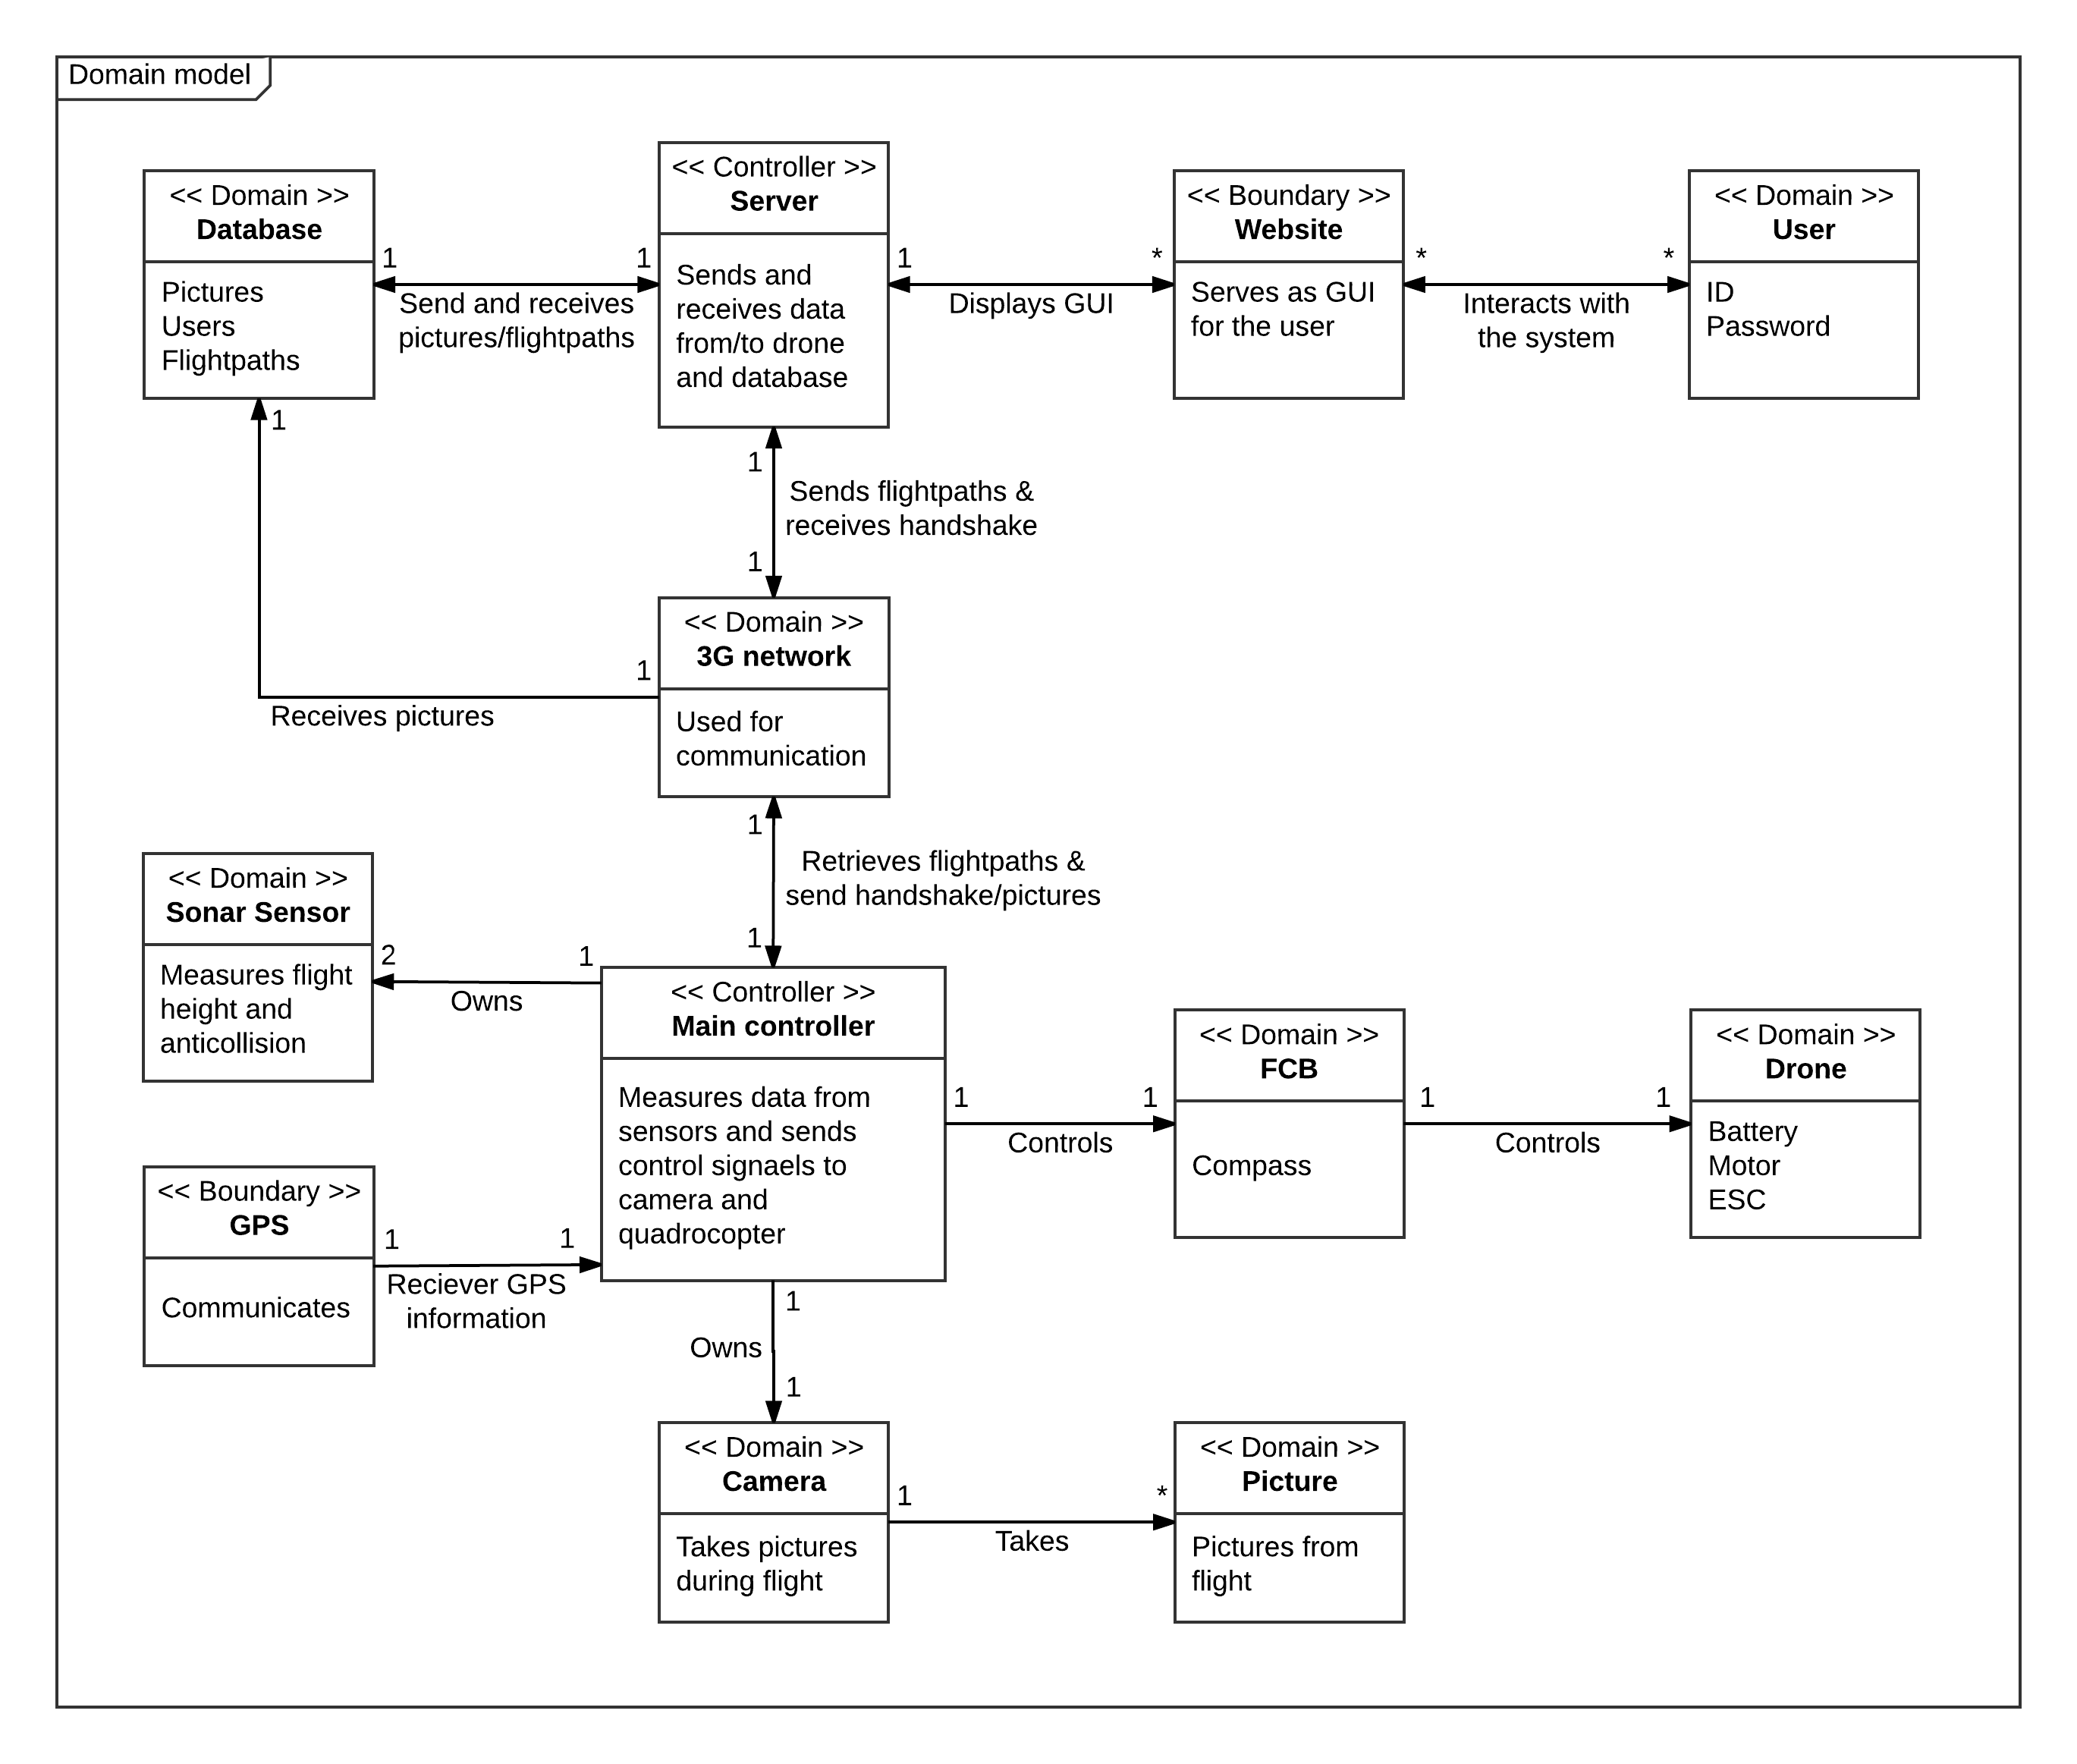
\includegraphics[width=1.\textwidth]{Billeder/domain_model.png}
	\caption{Domain model}
	\label{fig:domain_model}
\end{figure}

\newpage

Af figur \ref{fig:domain_model} ses det at domain modellen er opbygget af tre forskellige typer klasser. Nedenfor beskrives de tre forskellige klasser:

\textbf{Domain klasser}\newline
Domain klasser repræsenterer systemets domæne. Domain klasser er passive elementer, der er ansvarlige for væsentlige delparter af systemets funktionalitet.  

\textbf{Boundary klasser}\newline
Boundary klasser repræsenterer use case-aktører og aktørernes grænseflader til systemet. Boundary klasser er elementer der ligger i den yderste periferi af systemet. I nogle tilfælde er boundary klasser "front-end" elementer, der er designet til at udsende output samt at tage imod input fra systemets bruger. I andre tilfælde er boundary klasser "back-end" elementer der bruges til at hjælpe/understøtte controller klasser.

\textbf{Controller klasser} \newline
Controller klasser indeholder systemets domænelogik og står for at kontrollere systemets boundary og domain klasser. Desuden er controller klasserne ansvarlige for at håndtere input og output fra systemets boundary klasser.\\

\vspace{0.5cm}

Domain modellen bruges både til beskrivelsen af systemets hardware og software arkitektur. Men der gøres primært brug domain modellen i software arkitektur afsnittet. I software arkitekturen bruges domain modellen bla. til at danne grundlag for softwareklasser, klassenavne og klassernes indbyrdes forhold.








